\section{Automatic Pipeline Synthesis}
\begin{figure*}[htb]
\centering
  \begin{subfigure}[t]{0.8\textwidth}
  \centering
  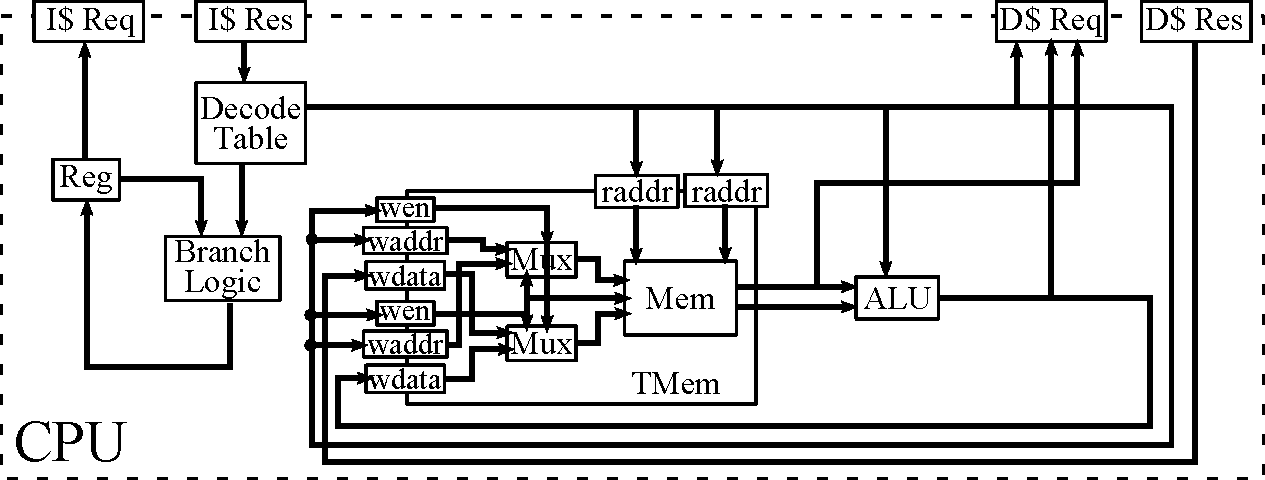
\includegraphics[width=\textwidth]{figures/pipeline.pdf}
  \caption{Datapath Graph.}
  \label{fig:datapathgrah}
  \end{subfigure}
  \begin{subfigure}[t]{0.8\textwidth}
  \vspace{20pt}
  \centering
  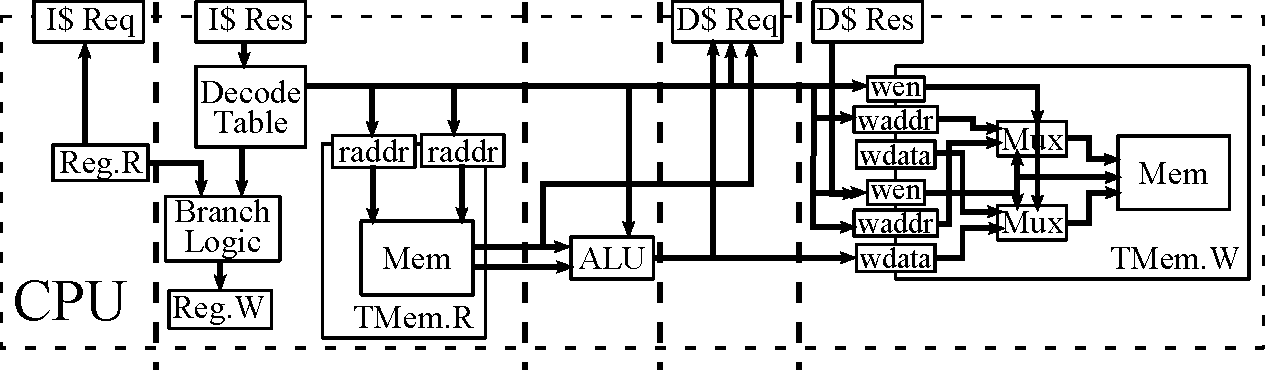
\includegraphics[width=\textwidth]{figures/pipelinedag.pdf}
  \caption{Datapath turned into a DAG.}
  \label{fig:datapathdag}
  \end{subfigure}
\caption{CPU Datapath}
\label{fig:datapath}
\end{figure*}

\subsection{Inserting Pipelines}

\subsection{Stage Coloring}

\subsection{Hazard Discussion}
\begin{figure*}[htb]
\centering
  \begin{subfigure}[t]{0.8\textwidth}
  \centering
  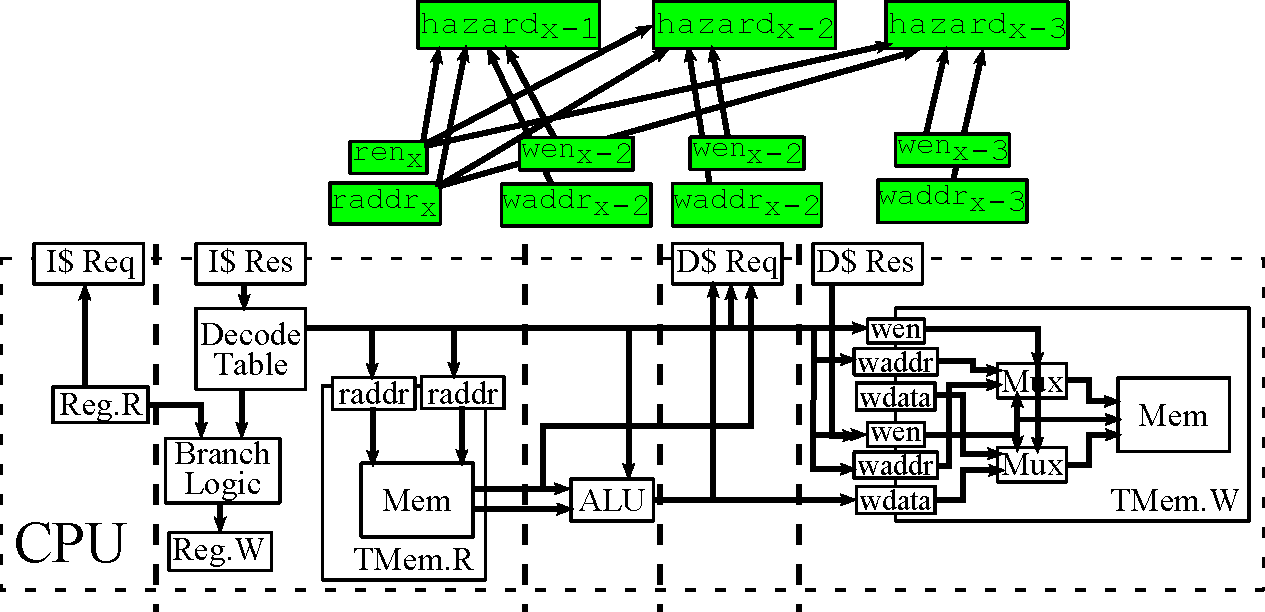
\includegraphics[width=\textwidth]{figures/pipelinehazard.pdf}
  \caption{Hazard Detection.}
  \label{fig:haz}
  \end{subfigure}
  \begin{subfigure}[t]{0.8\textwidth}
  \vspace{20pt}
  \centering
  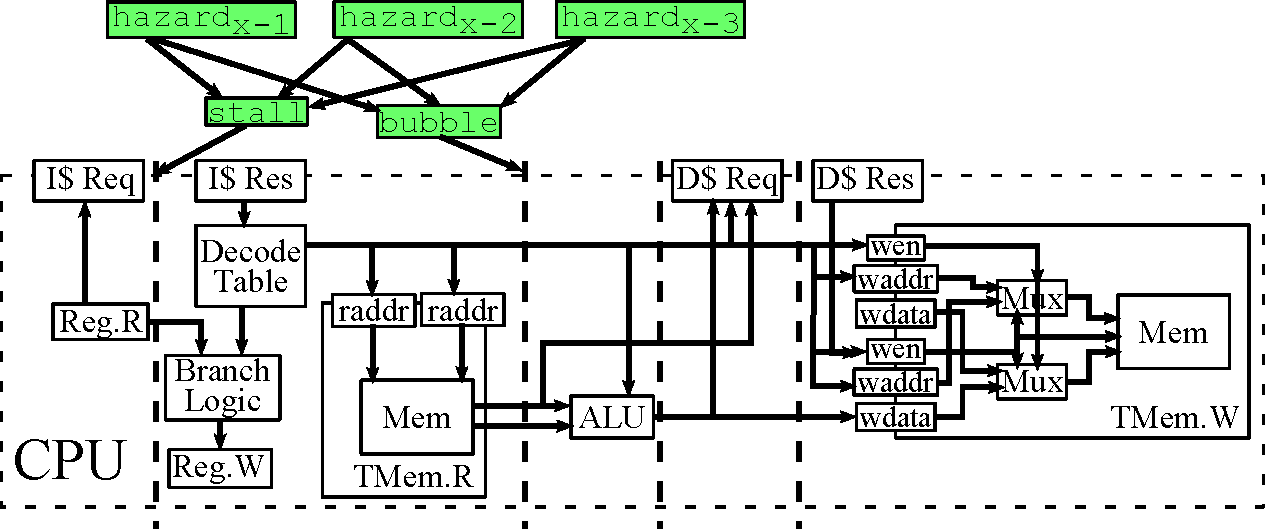
\includegraphics[width=\textwidth]{figures/pipelineinterlock.pdf}
  \caption{Interlocks.}
  \label{fig:int}
  \end{subfigure}
\caption{Resolving hazards through interlocks}
\label{fig:hazint}
\end{figure*}

{\bf Hazard Types}.

{\bf Detection}. Inserting pipeline registers into the datapath
graph introduces pipelining hazards that are not present in the
unpipelined datapath. Here we discuss how to handle data hazards which
result from a transaction reading a state element (a {\tt Reg} node or a
{\tt TransactionalMem}) before an earlier transaction writes to that state
element. 

We first search through the datapath graph to find all state
elements. For every state element, we determine whether or not a
hazard exists on it. If there is a hazard on a state element, we add
the hazard condition into a list. For {\tt Reg} or {\tt TransactionalMem}, a
hazard condition exists if the state element belongs in a stage that precedes the
stage of its write enable or write data signal. The actual Boolean
hazard condition is {\tt wen \&\& ren} for a {\tt Reg} node and
{\tt wen \&\& ren \&\& waddr == raddr} for a {\tt TransactionalMem}.

Figure~\ref{fig:haz} shows the hazard conditions that our tool
identifies on the {\tt TransactionalMem}. when analyzing the generated pipeline in
Figure~\ref{fig:datapathdag}. We first search the pipeline for all
state elements. In this example, the {\tt Reg} node and the 
{\tt TransactionalMem} are the only state elements. We then examine
the read and write ports of these state elements to determine whether
or not there are any hazards. The {\tt Reg} has its write port in the
second stage but its read port is in the first stage. So we generate a
hazard signal in the first stage. The {\tt Transactionalmem} has its
write port in the fifth stage but its read port is in the second
stage. We trace backwards from the {\tt wen} in the fifth stage to the
second stage to find all the other {\tt wen} signals. For each 
({\tt wen}$_i$, {\tt waddr}$_i$) pair, we generate a hazard condition
{\tt wen$_i$ === ren$_i$ \&\& waddr$_i$ === raddr}.

\subsection{Hazard Resolution Options}
\begin{figure*}[htb]
\centering
  \begin{subfigure}[t]{0.8\textwidth}
  \centering
  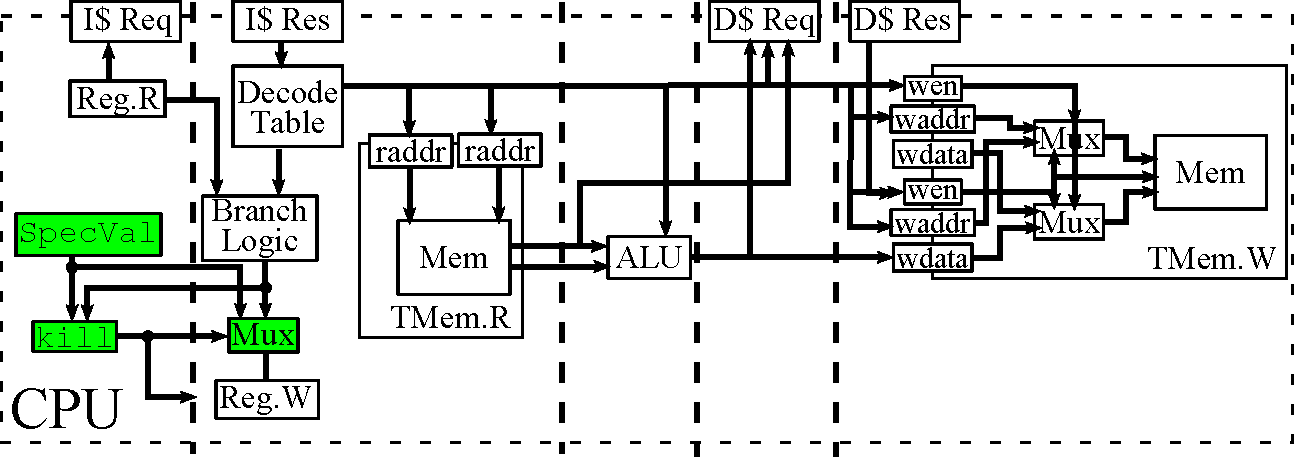
\includegraphics[width=\textwidth]{figures/pipelinespec.pdf}
  \caption{Speculation.}
  \label{fig:spec}
  \end{subfigure}
  \begin{subfigure}[t]{0.8\textwidth}
  \vspace{20pt}
  \centering
  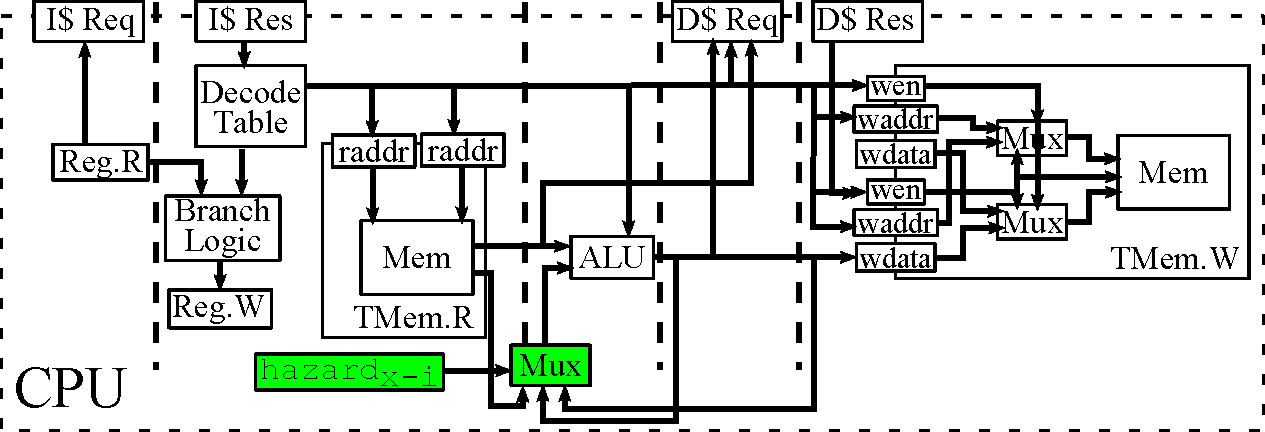
\includegraphics[width=\textwidth]{figures/pipelinebypass.pdf}
  \caption{Bypassing.}
  \label{fig:bypass}
  \end{subfigure}
\caption{Resolving hazards through speculation and bypassing}
\label{fig:specbyp}
\end{figure*}

{\bf Interlocks}. The easiest way to resolve
hazards is through interlocks. This hazard resolution method requires
no additional input from the user. Every identified hazard is placed
into the stage of the read port that generates the hazard. In
Figure~\ref{fig:haz}, the hazards would be placed into the second
stage because the corresponding read port is in the second stage. We
then go through every stage and perform an {\tt OR} reduction on all
the hazards in that stage as well as all the hazard conditions in the
following stages to produce the stall condition for that stage. The
second part of interlocking a pipeline is to push bubbles. We go
through every stage and generate a {\tt pushBubble} signal if there is
a hazard condition in that stage and no following stages have a
hazard.

Figure~\ref{fig:int} shows the interlock logic that our tool
generates to handle the hazards from Figure~\ref{fig:haz}. Since
the {\tt TransactionalMem}'s read port is in the second stage, all the
{\tt hazard$_i$}s go into the second stage. When examining the second
stage, the tool would {\tt OR} reduce all the {\tt hazard}$_i$s to
generate a stall condition to stall the first stage. The same hazard
condition is then used to generate the {\tt pushBubble} signal. There
are no other sources of hazards further down the pipeline so the
hazard condition in the second stage is sufficient for pushing a
bubble into the second stage.

{\bf Speculation}.

{\bf Bypassing}.
